\documentclass[tikz ,border=30pt]{standalone}
\usepackage{tikz}
\usetikzlibrary{fit,positioning, arrows, intersections}
\usepackage{verbatim}
\begin{document}
\centering
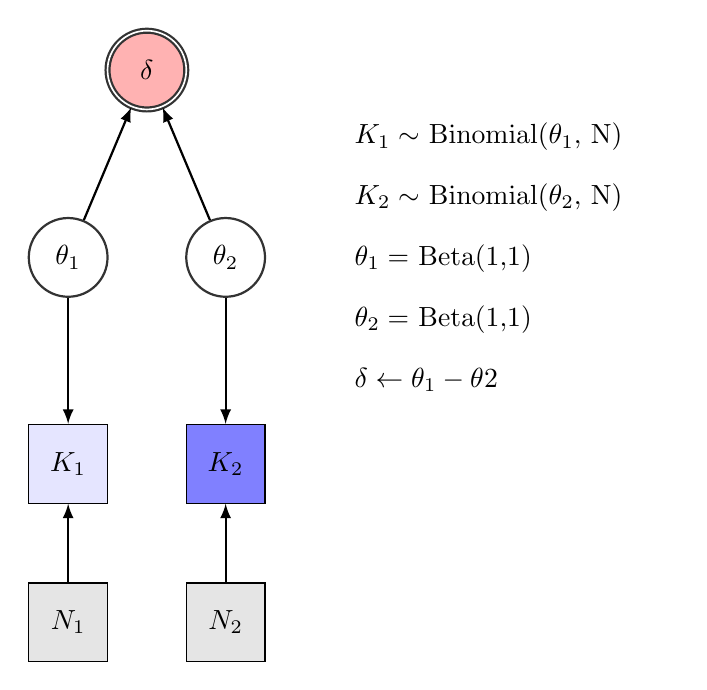
\begin{tikzpicture}
\tikzstyle{circ}=[circle, minimum size = 10mm, thick, draw =black!80, node distance = 16mm]
\tikzstyle{connect}=[-latex, thick]
\tikzstyle{sqr}=[rectangle, draw=black!100, minimum size=10mm]
\baselineskip=32pt
% 2. Nodes
%%%%%%%%%%
\node[sqr, fill=blue!10] (K1) at (1,0) {$K_1$};
\node[sqr, fill=black!10] (N1) [below=of K1] {$N_1$};
\node[circ, fill=white!100] (theta1) [above=of K1] {$\theta_1$};

\node[sqr, fill=blue!50] (K2) at (3,0) {$K_2$};
\node[sqr, fill=black!10] (N2) [below=of K2] {$N_2$};
\node[circ, fill=white!100] (theta2) [above=of K2] {$\theta_2$};

\node[circ, double,fill=red!30] (delta) at (2,5) {$\delta$};

\node [text width=4cm] (dists) [right=of theta2] {
          $K_1 \sim $ Binomial($\theta_1$, N)\\[1em]
          $K_2 \sim $ Binomial($\theta_2$, N)\\[1em]
          $\theta_1 = $ Beta(1,1)\\[1em]
          $\theta_2 = $ Beta(1,1)\\[1em]
          $\delta \leftarrow \theta_1 - \theta2$
          } ;
% 3. Arrows
%%%%%%%%%%%
\path (N1)      edge [connect] (K1)
      (theta1)  edge [connect] (K1)
      (N2)      edge [connect] (K2)
      (theta2)  edge [connect] (K2)
      (theta1)  edge [connect] (delta)
      (theta2)  edge [connect] (delta);

\end{tikzpicture}

\end{document}